%%%%%%%%%%%%%%%%%%%%%%% file moduleX_template.tex %%%%%%%%%%%%%%%%%
%
%
% This is a template for creating your papers for the course KRW
% It is based on the standard Latex template for Springer publications
% but contains a suggestion for the structure and some content of the
% paper.
%
% Please adapt this document wherever needed.
%
% For more information about the required Latex Style check the document
% typeinst.pdf in the StyleFiles directory.
%
%%%%%%%%%%%%%%%%%%%%%%%%%%%%%%%%%%%%%%%%%%%%%%%%%%%%%%%%%%%%%%%%%%%%%%%%%


\documentclass[runningheads,a4paper]{../../StyleFiles/llncs}

\usepackage{url}
\usepackage{graphicx}
\usepackage{amssymb}
\usepackage{listings}
\lstset{language=SQL,morekeywords={and, some, exactly}}
\usepackage{caption}
\usepackage{subcaption}
\captionsetup{compatibility=false}

\newcommand{\keywords}[1]{\par\addvspace\baselineskip
\noindent\keywordname\enspace\ignorespaces#1}

\begin{document}

\mainmatter  % start of an individual contribution

% first the title is needed
\title{Data- and Ontology Paper: Quality Ontology for Handicap Parking Spots around Venues in Amsterdam}

% a short form should be given in case it is too long for the running head
\titlerunning{Data- and Ontology Paper}

% the name(s) of the author(s) follow(s) next
%
% NB: Chinese authors should write their first names(s) in front of
% their surnames. This ensures that the names appear correctly in
% the running heads and the author index.
%
\author{Alivanistos, Dimitris. \\ Baez, Selene. \\ Jemmett, Andrea. }
%
\authorrunning{Alivanistos, Dimitris. \\ Baez, Selene. \\ Jemmett, Andrea.}
% (feature abused for this document to repeat the title also on left hand pages)

% the affiliations are given next; don't give your e-mail address
% unless you accept that it will be published
\institute{\url{d.alivanistos@student.vu.nl} \and \url{s.baezsantamaria@student.vu.nl} \and \url{a.jemmett@student.vu.nl}}

\maketitle


\begin{abstract}
We introduce a Linked Dataset integrating three different datasets related to the city of Amsterdam. We present the details of the dataset and the ontology that we introduce to cover all the important concepts of those data. Also we provide a thoughtful analysis of the methodology that we applied and the evaluation techniques that have been embraced. We enhanced our previous dataset with a richer ontology and we show how we published our results following the 5-star model for Linked Data.
\end{abstract}

\section{Introduction}
Amsterdam, a busy and tourist city as it is, offers a variety of events throughout the year. As such, a relevant topic related to the previous is the accessibility the city provides for handicap people to attend such events. In particular, this project focuses on providing these users with a way to find Parking Slots when attending events in different venues in Amsterdam.

Though information about handicap parking slots in Amsterdam is public through the Municipality, the datasets are not structured in a human readable manner. Moreover, the link to venues and events is not well organized and has not been addressed in a user-friendly manner. To the extent of our knowledge, the application that gets closest to this description is the official website for Accessibility in Amsterdam, which still fails to provide with an easily searchable tool for finding handicap parking slots given an Event and/or Venue.
%TODO link to download datasets and to website.

This paper is an extension of the previous paper on Milestone 1, where we set up the project to solve the aforementioned problem, linking datasets from events at Theatres, and Museums and Galleries, to the Handicap Parking Slots dataset. In this paper the overall goal is to improve on the knowledge graph created for the application by creating an ontology that is formal yet intuitive for its potential users.

In the following section we further motivate the paper by providing concrete use cases that lead to a list of higher level requirements to be fulfilled by our project. Later, we describe an inspiration paper that guided us through the design of our ontology. We continue to describe our ontology, highlighting the major improvements from the knowledge graph in Milestone 1, followed up by evaluating the proposed ontology. Finally, some discussion provides with insights regarding the main contributions and future improvements on this project.

\section{Use Case and Requirements}
%\textit{Describe the use-case you have in mind that motivates the need for the ontology. This could be the original use case from milestone 1, but then you should explain why the schema you defined previously falls short. What requirements should the ontology meet? What is its intended scope.}
In order to better illustrate the motivation for this project we look back to the use cases from Milestone 1 to evaluate how well the current knowledge graph meets their needs. Next, we ambitiously create a couple more use cases to extend the potential uses of the application. We finalize by providing with a list of three specific requirements an ontology must meet to satisfy the users needs.

\subsection{Previous use cases}
\begin{enumerate}
	% Planning in advance
	\item John is in a wheelchair and wants to go to an exhibition in Van Gogh Museum Friday night. The day before the show, John uses our application to find the parking slots closest to the museum and heads to the show confidently. 
	% Quick search once in the theater (on the fly)
	\item Peter broke his leg last month and his friends, as an attempt to cheer him up, invited him to come to a comedy show at the Comedy Cafe. He is quite late and quickly browses our application and finds an area with several parking slots. He drives in that direction hoping to find an available slot. 
	% Event manager
	\item Mary is an event organizer who wants to host an exhibition in a museum next month. She is looking for an accessible venue so she would like to see the distribution of parking slots around the main galleries in Amsterdam. She has a list of five places in mind and uses our application to explore and choose the best venue.
\end{enumerate}

\subsubsection{Reflection on previous knowledge graph} 
In the previous Milestone we showed that our application successfully integrates the Events and Handicap Parking Slots datasets, thus allowing users to look for parking slots close to venues in a time-saving way. However, some of the needs expressed in the previous use cases can be better met. For example, currently John and Peter would have to browse through a long list of events till they find the exhibition or show they are attending. A better ontology that subdivides events into types could help them navigate the data more easily. 

Furthermore, another notable shortcoming is that parking slots are only sorted in terms of distance to venues, ignoring other relevant facts like its size. For example, Peter might want to head to a close, yet large parking slot in order to increase its chances to find an available spot. Similarly, Mary might want to have information about the capacity of the parking slots depending on the size of the event she is planning.

\subsection{New use cases}
\begin{enumerate}
	% Search by interest
	\item Toby is a Theatre fan and he is interested in watching as many plays as possible. He is in a wheelchair and needs accessible parking spots to go to Theatres when he selects a play to watch. 
	% Search by area
	\item Chelsea has appointments once every week at the Femme Amsterdam Hospital. She would like to look for events nearby to attend after her sessions. 
\end{enumerate}

\subsection{Requirements}
\label{requirements}
Given the above, we abstract the users needs into a high level set of requirements. To keep the project within a manageable scope, we limit the requirements to three items, summarized in the following list.

\begin{enumerate}
	\item A user should be able to look for specific types of events or specific venues according to his/her interests.
	\item Information about the size of the parking slots should be readily available through search. 
	\item Events, Venues and/or Parking Slots within a certain area should be related to each other and they can be easily grouped. 
\end{enumerate}


\section{Related Work}
%\textit{What other ontologies did you find that cover a similar domain. To what extent can they be reused. Have others (e.g. other students) developed similar datasets/ontologies that feed/meet your requirements, where do they fall short? Papers to look for are published at eg. ISWC, ESWC, EKAW and FOIS, or the Journal of Web Semantics, and the Semantic Web Journal.}
While doing research to meet the previous requirements, we ran across a variety of ontologies that aim to cover similar domains as ours. Within the domain of information related to cities, we found the work by Komninos et al.\cite{komninos2015smart} to be particularly inspirational for designing this paper's ontology. With its project, the authors bring awareness to the fact that, regardless of the effort by developers to create applications for smart cities, the impact of those is still low. They attribute the problem to the lack of coordinated effort to create a standardized high quality ontology, and propose to unify the existent ontologies into the Smart City Ontology (SCO).   %Following a structure thinking, SCO consists of 10 superclasses which reflect the three main aspects of a smart city. 

We want to accentuate the importance of coordination among well-formed ontologies and so we designed our ontology with the thought in mind to fit the broader schema laid down by Komninos el al. Ours is a specific and relatively small ontology that focuses on Handicap Parking Slots, Venues and Events. Yet, its full of potential can be achieved when assembled together with ontologies regarding other aspects of a city. 

\section{Methodology}
%\textit{Describe the methodology you followed for constructing the ontology. How did you guarantee that the ontology meets the needs and requirements of the use case? Have you used any existing design patterns, partial ontologies, competency questions etc.}

Given the requirements from Section \ref{requirements}, and with the objective mentioned above, we design the ontology through an iterative process, revising at each step that the users needs were met while keeping the potential for linking to other ontologies open. We use Protege 5.0 as a tool for creating the ontology as well as for testing the inferences among the stated facts. 

Furthermore, we elaborate on the expressiveness of the ontology and exploit the power of the Web Ontology Language (OWL) to represent more complex aspects such as cardinalities and equivalences among existing and newly created Subclasses and Object Properties.

As stated in the previous Milestone, we incorporate other ontologies like \texttt{DBpedia} \footnote{The \texttt{DBpedia} namespace is defined at \url{http://dbpedia.org/ontology/}} for location management, and \texttt{geo} \footnote{The \texttt{geo} namespace is defined at \url{http://www.w3.org/2003/01/geo/wgs84_pos}} for latitude and longitude management. This time, we exploit the usage of DBpedia and make use of the equivalence between dbo:Place and dbo:Location. Further explanation of the benefits of this are explained in the following section.

\section{The Ontology}
%\textit{Systematically describe the ontology and highlight the (interesting) design choices you had to make. Were there things you wanted to represent but couldn't given the limitations on the KR language?\footnote{If you do not encounter any limitations, you should be more ambitious about the model!} How did you work around these limitations? (integrity constraints, additional rules?) Describe how the ontology meets the 5 star model for Linked Vocabulary Use.}
A comparison between the old knowledge graph (Figure \ref{fig:old_ontology}) and the newly created ontology (Figure \ref{fig:ontology-classes}) is graphically depicted below. 

\begin{figure}[h]\centering
	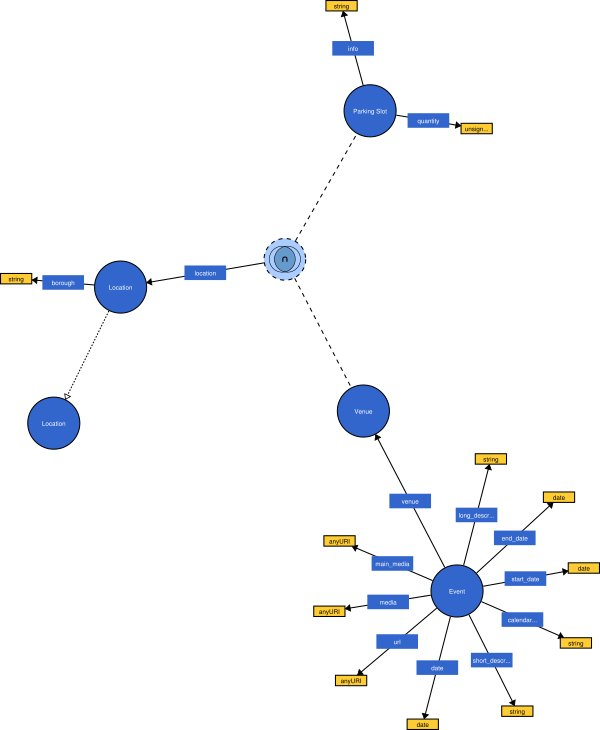
\includegraphics[width=.7\textwidth]{img/old_ontology.jpg}
	\caption{Knowledge graph from Milestone 1.}
	\label{fig:old_ontology}
\end{figure}
\begin{figure}[h] \centering
	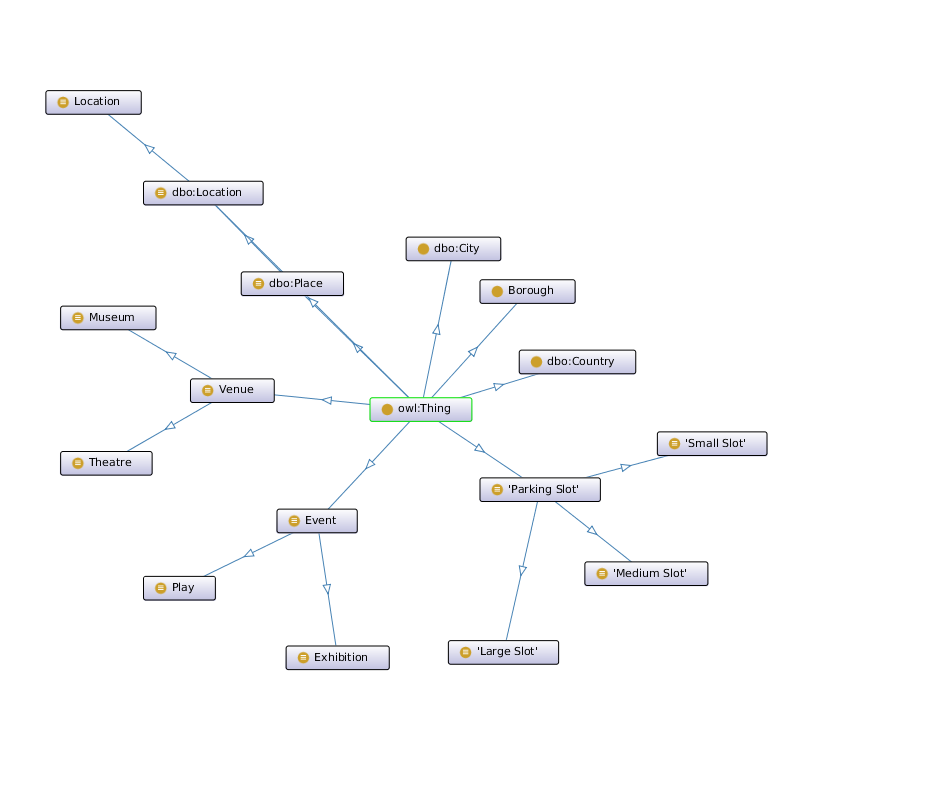
\includegraphics[width=.7\textwidth]{img/ontology-classes.png}
	\caption{Class hierarchy for the current version of the Find A Slot ontology.}
	\label{fig:ontology-classes}
\end{figure}

Given the degree of variation between both ontologies, we divide the updates on Entities and Properties and give a more detailed explanation in the following subsections.

\subsection{Entities}
The main difference with the previous version of the ontology is that each of the three main classes is now subdivided into more specific subclasses. For example:
\begin{itemize}
	\item \textbf{Events}: Divided into Plays and Exhibitions
	\item \textbf{Venues}: Divided into Theatres and Museums
	\item \textbf{Parking Slots}: Divided into Small, Medium and Large Slots
\end{itemize}

The divisions for the first two come straight from the datasets themselves. On the one hand, when an event comes from the Theatres dataset, we assume it is of type Play and it happens in a Venue of type Theatre. On the other hand, when the event comes from the Museums and Galleries dataset, we assume it is of type Exhibition and it happens in a Venue of type Museum.

The third one, however, is a distinction we propose in order to better describe the Parking Slots. Previously, a Parking Slot's capacity was only described by its Datatype Property \textit{Quantity}. Now, we take this property and process it to classify Parking Slots into three types: Small (consisting on 1 or 2 individual slots), Medium (consisting of 3 or 4 individual slots) and Large (consisting of 5 or more individual slots). This classification is achieved through an equivalence fact as exemplified by the next listing. \\

\begin{lstlisting}[captionpos=b, caption=Definition of Large Slot a subclass of Parking Slot, label=lst:owl, basicstyle=\ttfamily\small,frame=bt,showstringspaces=false]
'Parking Slot' 
and (quantity some xsd:unsignedInt[>= "5"^^xsd:unsignedInt])
\end{lstlisting}

\begin{lstlisting}[captionpos=b, caption=Definition of Medium Slot a subclass of Parking Slot, label=lst:owl, basicstyle=\ttfamily\small,frame=bt,showstringspaces=false]
'Parking Slot' 
and (quantity some xsd:unsignedInt[>= "3"^^xsd:unsignedInt,
 < "5"^^xsd:unsignedInt])
\end{lstlisting}

\begin{lstlisting}[captionpos=b, caption=Definition of Small Slot a subclass of Parking Slot, label=lst:owl, basicstyle=\ttfamily\small,frame=bt,showstringspaces=false]
'Parking Slot' 
 and (quantity some xsd:unsignedInt[>="1"^^xsd:unsignedInt ,
  < "3"^^xsd:unsignedInt])
\end{lstlisting}

The last extension of the entities regards the creation of a class for \textit{Borough} with the purpose of linking it to our Location entity. As explained before, we use the DBpedia ontology for the management of locations. However, dbo:Location does not include Boroughs, a crucial part of the description of a  location in Amsterdam. Thus, we create a subclass called Location, which is equivalent to a dbo:Location with a Borough, to represent the specific case of locations in Amsterdam.

\subsection{Properties}

The first extension in the Properties regards restrictions on datatype properties. We have included cardinalities with respect to the real world. An example can be seen at the Event entity where we state that an Event must have at least one Venue where it will take place.

Furthermore, we introduced the 'Event venue' property which has sub-properties 'Exhibition Venue' and 'Play Venue' according to their range. If event is an Exhibition then it uses the 'Exhibition Venue' property. We have also introduced the 'Venue Events' property as the inverse property of 'Event venue'. 

Moreover we included in our dbo:location property two sub-properties named 'slot location' and 'venue location'. We use these properties to restrict our dbo:location to have domain Parking Slot when we use the 'slot location' property and Venue when we use the 'venue location'. Both of them have Location as range.

The last extension of our properties section refers to the addition of the properties \textit{Borough} , \textit{City} and \textit{Country}. The reason behind this is that we want to have restrictions. In order to ensure that a dbo:location has exactly one country we use the equivalent rule: \\

\begin{lstlisting}[captionpos=b, title=Class equivalent to dbo:Location with the use of our subproperties, label=lst:owl, basicstyle=\ttfamily\small,frame=bt]
(city exactly 1 dbo:City) 
and (country exactly 1 dbo:Country) 
and (address exactly 1 xsd:string)
\end{lstlisting}

Similarly for our \textit{Location} the equivalent rule is: 

\begin{lstlisting}[captionpos=b, title=Class equivalent to Location with the use of our subproperty borough, label=lst:owl, basicstyle=\ttfamily\small,frame=bt]
dbo:Location 
and (dbo:borough exactly 1 Borough)
\end{lstlisting}

\section{The Dataset}
% Describe how you recasted the dataset(s) of the previous assignment to the new ontology (perhaps you found other datasets that you want to add). What did it take to do this? What metadata have you published alongside the dataset, and how did you generate it? (Provenance, VOID, etc.) Describe how your data meeds the 5 star model for Linked Data.
Once again, the three datasets have been converted to a linked data format, now using the second version of the ontology in a straightforward way. We create resources for the newly introduced \texttt{Borough} class. Cities and countries have been recasted to point to DBpedia resources. Entities of class \texttt{Museum} or \texttt{Theatre} are created based on their original dataset of provenance. An \texttt{Event} is linked to a \texttt{Venue} via a newly created object property and this allows the reasoning engine to infer if an \texttt{Event} is a \texttt{Play} or an \texttt{Exhibition} based on its Venue type.

Given the quantity of slots available for a \texttt{ParkingSlot}, thanks to the new ontology, the dataset distinguishes parking slots based their availability into \texttt{SmallSlot}, \texttt{MediumSlot} and \texttt{LargeSlot}. This provides a richer classification of parking slots than based on the quantity
property directly. It is remarkable that we get this through inference since it has not been directly coded into the conversion script.

Each of the three datasets has been published with its companion VoID dataset, describing the contents of the dataset it refers to. Most of the metrics and metadata have been generated using \textbf{rdflib}'s \texttt{generateVoID} method applied on the three graphs. Moreover we publish a VoID Linkedset that links together the three datasets as a new one. Alongside, we provide some additional metadata from the \texttt{void:}\footnote{\url{http://rdfs.org/ns/void#}} ontology -such as \texttt{target}, \texttt{sparqlEndpoint} and \texttt{exampleResource}- and from the \texttt{dcterms:}\footnote{\url{http://purl.org/dc/terms/}} ontology -such as \texttt{subject}, \texttt{title} and \texttt{description}. Those additional metadata have been added manually to the VoID dataset. The \texttt{void:Linkset} can be retrieved at the following URL \url{http://data.krw.d2s.labs.vu.nl/doc/group6/findaslot/resource/findaslot/void}.

\subsection{5-star Open Data}
We say that the published database meets the standards proposed by the 5-star model for Linked Data \cite{janowicz2014five}. Here we defend our statement by taking each of the five steps into consideration.

\begin{description}
\item[Available on the Web] We published our data under an open license, namely the CC0 1.0 Universal (this is declared in the VoID metadata).
\item[Available as structured data] The dataset is available in RDF format which is structured.
\item[Available as non-proprietary format] Our dataset is specified in a W3C language so it is not in a proprietary format but in an open and standardized format.
\item[Use URIs to denote things] We use URIs to denote everything that is not an RDF Literal. Events, Venues, Locations and, starting from this version of the ontology, we include countries, cities and boroughs as resources defined by URIs.
\item[Link to other data] We provide external pointers to resources from DBpedia such as for cities (e.g. \texttt{dbr:Amsterdam}), countries (e.g. \texttt{dbr:Netherlands}) or as \texttt{dcterms:subject}, in the VoID
specification, we point to \texttt{dbr:Museums} and \texttt{dbr:Parking\_space}.
\end{description}


\section{Evaluation}
For evaluating our ontology we got inspired by the work of Hlomani and Stacey \cite{hlomani2014approaches} on ontology evaluation and decided to evaluate our ontology using three major criterion:
\begin{enumerate}
	\item \textbf{Task-based Evaluation}. First of all we perform a task-based evaluation that typically evaluates how effective our ontology is in the context of an application, using the list of Requirements from Section \ref{requirements} to do so. 
	\item \textbf{User-based Evaluation}. We perform a user-based evaluation that evaluates the ontology through user's experiences. Contrary to task-based evaluation, we are not accessing semantic validity and consistency of our ontology but we focus on the subjective information of it.
	\item \textbf{Data-driven evaluation}. In the last part of this section we focus on evaluating our ontology by comparing it with existing data about the domain it models.
\end{enumerate} 

\subsection{Task-based Evaluation}                                                                                                                                                                    
\begin{enumerate}
	\item \textbf{Search by interest:} With the extension of our ontology we succeed in extending our application. We have enabled the search by interests, as we initially divide Events and Venues with regard to personal interest. This way the users can narrow down their search avoiding non-essential information.
	
	\item \textbf{Search by area:} Another main aspect that adds to the improvement of our ontology is the detailed location information that users have access to. Now, users have the ability to search for Venues and Parking Slots in same Borough in a simple way.
	
	\item \textbf{Capacity of Parking Slots:} We also provide with explicit information about each Parking Slot that is close to the interests of the user. Users now have prior knowledge regarding the capacity of the parking spot they need, increasing their chances of finding an available slot.
\end{enumerate}

\subsection{User-based Evaluation}
For our user-based evaluation we simply examined our dataset as a \textit{third party user}. The source and the metadata that have been added with the void ontology provide with important information, not only on each of the three datasets separately but on the integrated dataset as a whole. \textit{Labels}, \textit{descriptions} and important \textit{metrics}, such as the total number of triples that exist in each dataset are only some of the metadata information that have been added. This way, a third party user is able to get information about our ontology directly, without having to query it himself, thus making our ontology an easy one to use by fellow ontology designers and developers.

\subsection{Data-driven evaluation}
So far our ontology combines knowledge from three different datasets in order to provide a useful service to the potential users of our application. Compared to other ontologies in the specific domain of finding parking slots it is clear that our ontology is quite innovative, since we focus specifically on people with a certain handicap. 

With the addition of Borough as a key feature of Location, the data can be combined in a more efficient way, increasing the total efficiency of our web application even further. Besides efficiency, we wanted to check how well our ontology \textit{fits the domain knowledge} \cite{brewster2004data}. 

This was done by comparing ontology concepts derived from the three separate datasets that we used in Milestone 1, with the latest version of our dataset. So far our ontology perfectly fits the domain knowledge of Handicap Parking Spots in Amsterdam, given by the three chosen datasets; however we acknowledge that there is certainly room for further improvement in the general domain of Events and Parking Slots.

\section{Discussion}
%\textit{Here you summarize the preceding sections, describe the lessons learnt and discuss future work.}
In this paper we provided a detailed description of the improved ontology that we have published about three datasets related to the city of Amsterdam. Moreover we show the methodology that we adopted and how this led our ontology to be classified as fully conform with the 5-star model for Linked Data.

Being conform to this model for Open Data means that publishers will ultimately have a dataset that is easily \textit{surfable} and \textit{connected} to other Web resources, generating more incoming traffic towards the dataset and increasing the value of the contained data. The 5-star model is a way to introduce sources of \textit{trust} in both the data and publishers' spaces. In particular we have found the set of propositions offered by the VoID framework to be very useful and powerful. Furthermore, we got experience on how easy it is to define \textit{discoverable} ontologies using Web standards.


\bibliographystyle{plain}
\bibliography{mybib}

\end{document}
